\documentclass[12pt, a4paper]{article}

\usepackage[czech]{babel}
\usepackage{lmodern}
\usepackage[utf8]{inputenc}
\usepackage[T1]{fontenc}
\usepackage[pdftex]{graphicx}
\usepackage{amsmath}
\usepackage[hidelinks,unicode]{hyperref}
\usepackage{float}
\usepackage{listings}
\usepackage{tikz}
\usepackage{xcolor}
\usepackage[final]{pdfpages}


\definecolor{mauve}{rgb}{0.58,0,0.82}
\usetikzlibrary{shapes,positioning,matrix,arrows}

\newcommand{\img}[1]{(viz obr. \ref{#1})}

\definecolor{pblue}{rgb}{0.13,0.13,1}
\definecolor{pgreen}{rgb}{0,0.5,0}
\definecolor{pred}{rgb}{0.9,0,0}
\definecolor{pgrey}{rgb}{0.46,0.45,0.48}

\lstset{frame=tb,
  language=C,
  aboveskip=3mm,
  belowskip=3mm,
  showstringspaces=false,
  columns=flexible,
  basicstyle={\small\ttfamily},
  numbers=none,
  numberstyle=\tiny\color{gray},
  keywordstyle=\color{blue},
  commentstyle=\color{dkgreen},
  stringstyle=\color{mauve},
  breaklines=true,
  breakatwhitespace=true,
  tabsize=3
}


\let\oldsection\section
\renewcommand\section{\clearpage\oldsection}

\begin{document}
	% this has to be placed here, after document has been created
	% \counterwithout{lstlisting}{chapter}
	\renewcommand{\lstlistingname}{Ukázka kódu}
	\renewcommand{\lstlistlistingname}{Seznam ukázek kódu}
    \begin{titlepage}

        \centering

        \vspace*{\baselineskip}
        \begin{figure}[H]
        \centering
        
\includegraphics[width=7cm]{img/fav-logo.jpg}
        \end{figure}

        \vspace*{1\baselineskip}

        \vspace{0.75\baselineskip}

        \vspace{0.5\baselineskip}
        {Semestrální práce z předmětu KIV/OS}

        {\LARGE\sc Simulace operačního systému\\}

        \vspace{4\baselineskip}

        \vspace{0.5\baselineskip}

        {\sc\Large Eliška Mourycová \\}
        \vspace{0.5\baselineskip}
        {A20N0061P}

        {\sc\Large Ondřej Drtina \\}
        \vspace{0.5\baselineskip}
        {A20N0077P}

        {\sc\Large Stanislav Král \\}
        \vspace{0.5\baselineskip}
        {A20N0091P}

        \vfill

        {\sc Západočeská univerzita v Plzni\\
        Fakulta aplikovaných věd}

    \end{titlepage}


    % TOC
    \tableofcontents
    \pagebreak

    
    \section{Analýza}
    % TODO analýza

    \section{Kernel}

    Kernel je část operačního systému, která provádí inicializaci hardwaru, zajišťuje správu prostředků a umožňuje vytvářet programy či vlákna. Uživatelskému prostoru nabízí své služby pomocí tzv. systémových volání. V této semestrální práci lze kernel rozdělit do následujících částí: 
\begin{itemize}
    \item správa procesů/vláken
    \item správa otevřených souborů
    \item souborový systém FAT12
\end{itemize}

\subsection{Správa procesů a vláken}
Tuto část kernelu lze považovat za nejdůležitější, jelikož bez její přítomnosti by nebylo možné spouštět žádné programy. Stará se o vytváření procesů a jejich správu, kdy lze procesy synchronizovat a nastavovat jejich návratové hodnoty. Simulace vláken a procesů je realizována pomocí konstrukcí pro vytváření vláken ze standardní knihovny \texttt{thread}. Většina kódu této části se nachází v souboru \texttt{/kernel/process.cpp}.

Pro použití služeb této části kernelu z uživatelského prostoru slouží následující systémová volání ze skupiny \texttt{Process}.

\begin{itemize}
    \item \texttt{Clone},
    \item \texttt{Wait\_For},
    \item \texttt{Read\_Exit\_Code},
    \item \texttt{Exit},
    \item \texttt{Register\_Signal\_Handler},
\end{itemize}

\subsubsection{Vytvoření nového vlákna}

Nativní identifikátory vytvořených vláken jsou mapovány na typ \texttt{kiv\_os::THandle}, který se dále používá v rámci kernelu jako interní identifikátor vláken.

Při zpracování požadavku na vytvoření nového vlákna se ze vstupních registrů načtou potřebné argumenty, a zavolá se funkce \texttt{run\_in\_a\_thread}, která přebírá argument obsahující vstupní bod části kódu, jež se má spustit v novém vlákně. Tato funkce vytvoří nové \texttt{std::thread} vlákno, kterému jako vstupní funkci nastaví funkci \texttt{thread\_entrypoint} přebírající skrz argumenty vstupní bod kódu ke spuštění. Uvnitř spuštěného vlákna se před vykonáváním kódu dále čeká dokud kernel nepřidá toto vlákno do tabulky všech vláken. Čekání je realizováno pomocí semaforu, a teprve po jeho notifikaci se začne vykonávat požadovaný kód. 

Při vytváření nového vlákna se navíc ještě dohledává jaké vlákno či proces nové vlákno vytváří. Tato informace se později např. využívá při změně pracovního adresáře procesu.

\subsubsection{Synchronizace vláken}
Jádro umožňuje synchronizaci vytvořených vláken pomocí systémového volání \texttt{Wait\_For}. Obsluha tohoto volání je realizována pomocí funkce \texttt{wait\_for}, která přebírá pole obsahující identifikátory vláken, na která se má čekat. Synchronizace je realizována pomocí semaforů, kdy ke každému běžícímu vláknu je veden seznam semaforů, které se mají při skončení vlákna notifikovat. Jeden semafor může tedy být přiřazen k více než jednomu vláknu. 

Na začátku obsluhy je k daným vláknům přiřazen nově vytvořený semafor, a zahájí se čekání na notifikaci tohoto semaforu. V moment, kdy je daný semafor notifikován, je vlákno čekající na semafor probuzeno, a tento semafor je odebrán ze všech ostatních seznamů, kde se vyskytuje. Spolu s notifikací semaforu je čekajícímu vláknu předána i informace o tom, jaké vlákno semafor probudilo. 

\begin{figure}[!ht]
\centering
{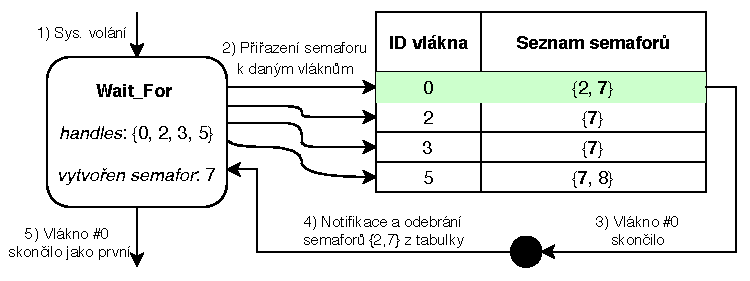
\includegraphics[width=14.5cm]{pdf/wait_for.pdf}}
\caption{Zjednodušený diagram obsluhy sys. volání \texttt{Wait\_For}}
\label{fig:screen-transition-diagram}
\end{figure}

\subsubsection{Vytváření procesů}
Vytváření procesů je principiálně stejné jako vytváření vláken a používá se stejných funkcí jako při vytváření nového vlákna. Hlavním rozdílem je to, že až v jádře se převádí název programu na vstupní bod programu, který se předává funkci \texttt{run\_in\_a\_thread}. Před zahájením vykonávání kódu programu je po vytvoření nového vlákna dle jeho identifikátoru přidán nový záznam do tabulky všech procesů. Dále taky nový proces dědí pracovní adresář od procesu, kterým byl vytvořen.

\subsubsection{Nastavení návratové hodnoty procesu}
Všem procesům je při jejich vytvoření nastaven výchozí návratový kód \texttt{kiv\_os::NOS\_Error::Success}. V případě, že nějaký program chce tento kód nastavit ručně, tak má možnost použít systémové volání \texttt{Exit}, a v registrech nastavit požadovaný návratový kód.

% TODO implementační část

    % ukázka kódu
    \subsection{Modul 1}
    	    \begin{lstlisting}[language=C, caption={Lorem ipsum dolor sit amet},captionpos=b]<F2>
#include <iostream>
using namespace std;

int main()
{    
    int divisor, dividend, quotient, remainder;

    cout << "Enter dividend: ";
    cin >> dividend;

    cout << "Enter divisor: ";
    cin >> divisor;

    quotient = dividend / divisor;
    remainder = dividend % divisor;

    cout << "Quotient = " << quotient << endl;
    cout << "Remainder = " << remainder;

    return 0;
}\end{lstlisting}


\section{Závěr}	
% TODO závěr

\end{document}    
